\documentclass[11pt]{report}
\usepackage{graphicx}
\usepackage{hyperref}
\usepackage{amsmath}
\usepackage{amssymb}
\usepackage{mathcomp}
\usepackage[english,spanish]{babel}
\usepackage{sectsty}
\usepackage{dirtytalk}
\usepackage{listings}
\usepackage{float}
\usepackage{apacite}
\graphicspath{ {./Media/} }

\usepackage{tikz}
\usetikzlibrary{automata,positioning}
\usepackage{pgfplots}

\bibliographystyle{apacite}

\usepackage{textcomp}

\newcommand{\sfdagger}{{\sffamily\textdagger}}

\chapternumberfont{\Large}
\chaptertitlefont{\LARGE}

\usepackage[symbol]{footmisc}

\usepackage[tocflat]{tocstyle}
\usetocstyle{standard}
\usepackage{blindtext}

\lstset{
basicstyle=\small\ttfamily,
columns=flexible,
breaklines=true
}

\makeatletter
\renewcommand\tableofcontents{
  \null\hfill\textbf{\Large\contentsname}\hfill\null\par
  \@mkboth{\MakeUppercase\contentsname}{\MakeUppercase\contentsname}
  \@starttoc{toc}
}
\makeatother

\begin{document}

\begin{titlepage}
	\centering
	{\scshape\LARGE Coursera \par}
	\vspace{6.5cm}
	{\LARGE \textbf{Notes}\par}
	{\LARGE Neural Networks and Deep Learning \par}
	\vfill
	{\Large\itshape Carlos Garc\'ia Gon\'alez\par}
	\vspace{1cm}
	{\large April 2020 - June 2020 \par}
\end{titlepage}

\tableofcontents
\selectlanguage{english}
\newpage
\chapter{Neural Networks and Deep Learning}

\section{Week 1}
\subsection*{What is a Neural Network?}
The housing price prediction problem can be seen as the simplest of Neural Networks. First, lets start by assuming that the house pricing is only affected by its size.
\begin{center}
	\textit{Size x -> Neuron (does the determined function) -> Price y}
\end{center}
In this particular case, a Relu (Rectified Linear Unit) function \ref{fig:F1} is presented and is often seen in Neural Network examples. There can not be a house priced at \$0, hence the implementation of this type of function.
\begin{figure}
	\centering
	\begin{tikzpicture}
		\begin{axis}[
			domain=-3:5,
			]
			\addplot+[mark=none,red,domain=-3:0] {0};
			\addplot+[mark=none,red,domain=0:5] {x};
		\end{axis}
	\end{tikzpicture}
	\caption{Plot of an example Relu function} \label{fig:F1}
\end{figure}
A neural network is produced by taking many single neurons and by stacking them together. \\
Now let\'s add more variables for the same problem, the representation of the network would be similar to the following graph:
\begin{center}
	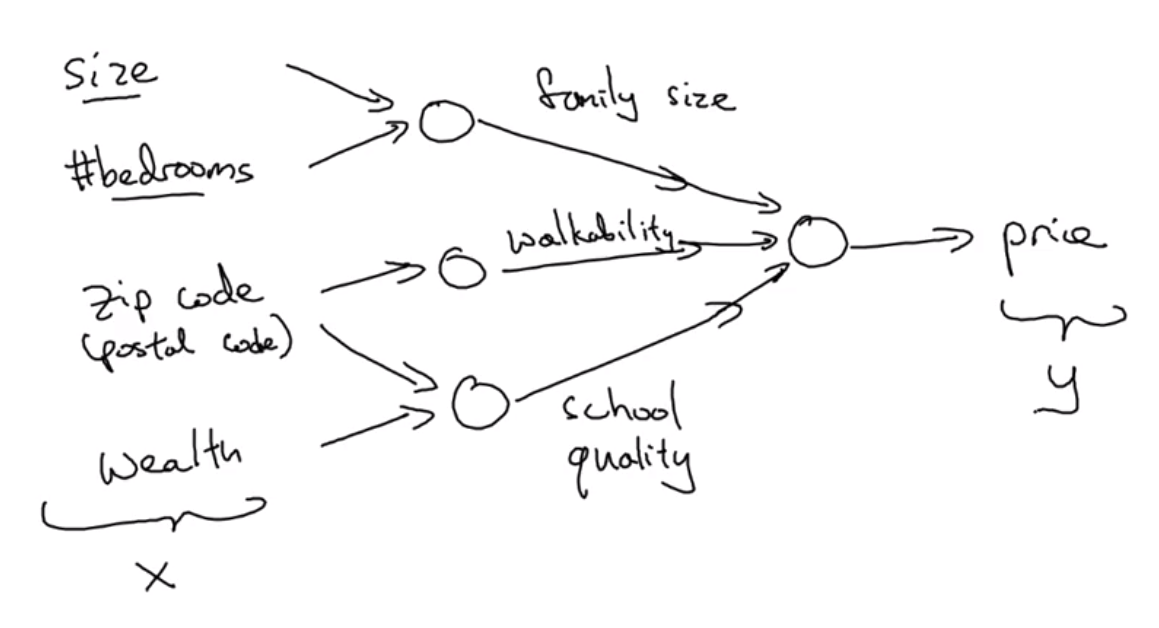
\includegraphics[width = .50\textwidth]{HPP.png}
\end{center}
The inter-connecting nods can be seen as individual Relu representations that lead to the values seen on the lines which represent important characteristics in a model and that lead to the final result; X is equal to the stack of the given inputs and Y is equal to the desired output. The \say{in-between} nods represent hidden features, these are the ones created subsequential to the input data and the network itself defines the relation between these.\\
The network receives three different types of data:
\begin{itemize}
	\item The X input values
	\item Training data
\end{itemize}
With these three the network can predict the output Y value. Giving a Neural Network enough correlational X:Y data will make it better at figuring out the sort of equations that are similar to the ones on the training data.

\subsection*{Supervised Learning}
Economic value of deep learning implementations really come from Supervised learning.
You have an input x and you want to have a result y. In the previous problem it would be x = Home features, y = Price and the application would impact on the real estate business. Another example could be related to e-marketing, where x = Ad \& user info, y = Click on add? (t/f) and the would impact on online advertising. Another examples could be related to computer vision, audio recognition, machine translation and other topic related projects. Simple neural networks such as the two first examples have usually a standard NN implementation, image processing is often convolutional and sequential data implementations (such as audio, because it has a temporal component) are often recursive NN; for particular or more complex implementations there can be custom or hybrid architectures.
\begin{center}
	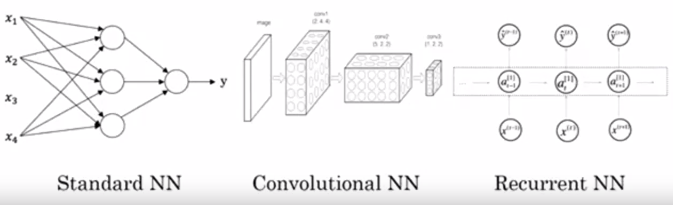
\includegraphics[width = .50\textwidth]{NNE.png}
\end{center}
Structured data (DB with specific fields) vs unstructured data (audio, images, [···]), this tangible difference is important to take into account because historically it has been more difficult to calculate from the latter, hence the importance of the architecture design importance. Although the most \say{exciting} implementations are often the unstructured data related systems, the market has more demand for well-built structured data solutions.

\subsection*{Why is Deep Learning taking off?}
in the traditional learning algorithms, there was a point where the increment of input data did nothing for the performance of the system. In modern problem solving we have a lot of data to handle, so the design of a system which could profit from it was considered crucial. Neural networks are capable of incrementing the system performance in a better fashion than traditional implementations. 
\begin{center}
	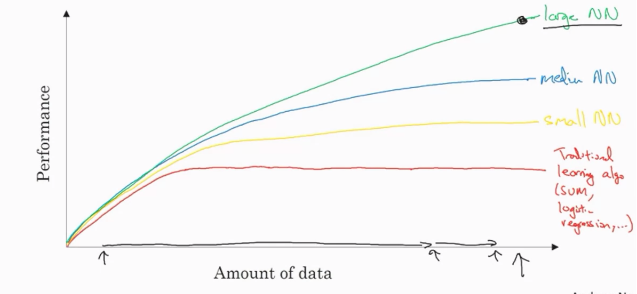
\includegraphics[width = .50\textwidth]{PRGR.png}
\end{center}
One thing to note is that the \say{Ammount of Data} refers only to the amount of labeled data (contains x and y definitions). Also, the notation for the cardinality is expressed as (m).\\
Although the increment in \say{learning room} is evident, the performance also has a cap that can occur if you run out of data or if the NN is big enough that it becomes really slow to train.\\
Large neural nets are only necessary when a lot of data is required to precess. There can be little to no difference in large NN and small NN systems where the data-set (m) is relatively small.\\
Deep learning progress has developed a weighted importance in data, computation-related (hardware-wise) and algorithmic advancements that allow the systems to come to a reality. One of the most notable innovations is the transition from sigmoid to RELU functions; sigmoid functions had areas (where b = 0) that led to the decrease of learning speed due to the slow parameter revision. The innovations of the three disciplines have helped the development cycle (idea -> code -> experiment) that leads to more architecture revisions.

\section{Week 2}

\subsection*{Binary Classification}
Usually the data processing is based on going through the entire dataset without explicitly using a for loop. Usually the process consists of a forward pause/forward propagation step, followed by a backward pause/backward propagation step.\\
Binary classification consists of an input x that is processed by an algorithm that outputs a binary value called label which indicates a certain input behavior or feature. For image classification (cat vs no cat), the image is decomposed to every pixel value per channel and then concatenated into a single object. \\
A single training example is denoted by the following notation:\\
$(x,y), x \in \mathbb{R}^{n_x}, y \in \{0,1\}$\\
The training set is comprised of all the pairs of training examples, lowercase m is commonly used as the indicator for the number of training examples.\\
In order to put the training examples in a more compact fashion, the following model must be used:
\begin{equation}
	X =
	\begin{Bmatrix} 
	\dots & \dots & \dots & \dots\\
	x^1 & x^2 & \dots & x^m \\
	\dots & \dots & \dots & \dots\\
	\end{Bmatrix} 
 \end{equation}
This matrix $X$ will have m columns, where m is the number of training samples and $n_x$ rows ($X \in \mathbb{R}^{n_x \times m}$). Although there are other implementations, using this convention will make further implementation easier.\\
For the label output, stacking the results in columns has also been commonly used, and is defined by the following model:
\begin{equation}
	Y =
	\begin{Bmatrix} 
	y^1 & y^2 & \dots & y^m
	\end{Bmatrix}
	, Y \in \mathbb{R}^{1 \times m} 
 \end{equation}

\subsection*{Logistic Regression}
Used when output labels are either 0 or 1. Given an input feature vector X you want an algorithm that can output a prediction which can be represented as \^y which is the estimate of Y. This before mentioned prediction is the probability $P(y=1 | x+
-)$.

\chapter{Improving Deep Neural Networks}

\chapter{Structure of Machine Learning Project}

\chapter{Convolutional Neural Networks}

\chapter{Natural Language Processing}

\bibliography{mybib.bib}

\end{document}
